
\documentclass{acm_proc_article-sp}
\makeatletter
\newif\if@restonecol
\makeatother
\let\algorithm\relax
\let\endalgorithm\relax
\usepackage{hyperref}
\usepackage[all]{hypcap}
\usepackage[usenames,dvipsnames]{xcolor}
\usepackage{listings}
\usepackage{algorithm2e}
%\usepackage{amsfont}
%\usepackage{amsmath}
%\usepackage{amssymb}
\hypersetup{
  bookmarks=true,         % show bookmarks bar?
  unicode=false,          % non-Latin characters in Acrobat’s bookmarks
  pdftoolbar=true,        % show Acrobat’s toolbar?
  pdfmenubar=true,        % show Acrobat’s menu?
  pdffitwindow=false,     % window fit to page when opened
  pdfstartview={FitH},    % fits the width of the page to the window
  pdftitle={My title},    % title
  pdfauthor={Author},     % author
  pdfsubject={Subject},   % subject of the document
  pdfcreator={Creator},   % creator of the document
  pdfproducer={Producer}, % producer of the document
  pdfkeywords={keyword1} {key2} {key3}, % list of keywords
  pdfnewwindow=true,      % links in new window
  colorlinks=true,       % false: boxed links; true: colored links
  linkcolor=cyan,          % color of internal links (change box color with linkbordercolor)
  citecolor=green,        % color of links to bibliography
  filecolor=magenta,      % color of file links
  urlcolor=cyan           % color of external links
}




\usepackage{listings}
\usepackage{algorithm2e}
\usepackage{verbatim}
\begin{document}
\title{Analysis of Security-Cost Trade-off of Fully Homomorphic Encryption Schemes}


%
% You need the command \numberofauthors to handle the 'placement
% and alignment' of the authors beneath the title.
%
% For aesthetic reasons, we recommend 'three authors at a time'
% i.e. three 'name/affiliation blocks' be placed beneath the title.
%
% NOTE: You are NOT restricted in how many 'rows' of
% "name/affiliations" may appear. We just ask that you restrict
% the number of 'columns' to three.
% Because of the available 'opening page real-estate'
% we ask you to refrain from putting more than six authors
% (two rows with three columns) beneath the article title.
% More than six makes the first-page appear very cluttered indeed.
%
% Use the \alignauthor commands to handle the names
% and affiliations for an 'aesthetic maximum' of six authors.
% Add names, affiliations, addresses for
% the seventh etc. author(s) as the argument for the
% \additionalauthors command.
% These 'additional authors' will be output/set for you
% without further effort on your part as the last section in
% the body of your article BEFORE References or any Appendices.

\numberofauthors{2} %  in this sample file, there are a *total*
% of EIGHT authors. SIX appear on the 'first-page' (for formatting
% reasons) and the remaining two appear in the \additionalauthors section.
%
\author{
\alignauthor
Kais Chaabouni \\
       \affaddr{ENSIMAG}\\
       \affaddr{Grenoble INP}\\
       \affaddr{Grenoble, France}\\
       \email{kais.chaabouni@ensimag.imag.fr}
% 2nd. author
\alignauthor 
Amrit Kumar\\
       \affaddr{ENSIMAG-Ecole Polytechnique}\\
       \affaddr{Grenoble INP}\\
       \affaddr{Grenoble, France}\\
       \email{amrit.kumar@ensimag.imag.fr}
}

% There's nothing stopping you putting the seventh, eighth, etc.
% author on the opening page (as the 'third row') but we ask,
% for aesthetic reasons that you place these 'additional authors'
% in the \additional authors block, viz.

\date{30 July 1999}
% Just remember to make sure that the TOTAL number of authors
% is the number that will appear on the first page PLUS the
% number that will appear in the \additionalauthors section.
\maketitle
\begin{abstract}
This paper investigates the feasibility of transformation of a (possibly) non-straight-line program (on unencrypted data) to a straight-line program on encrypted data. We present an analysis of security-cost trade-off for homomorphic encryption schemes on such programs. Analysis is based on the measurements (CPU time and  Wall time) taken for programs : performing \texttt{XOR} of an $n$-bit sequence, determining the majority bit of an $n$-bit sequence, evaluating the sum of $n$-bit integers, \textcolor{orange}{sum of integers with any number of bits} and sorting $n$ bit sequences of length $nbits$ (requires verifying the validity of a boolean predicate). The evaluation is performed on an available implementation ``Scarab library'' of a fully homomorphic encryption scheme. 

\end{abstract}

\keywords{ Fully Homomorphic Encryption, Security, Cost.} % NOT required for Proceedings

\section{Introduction}

The notion of \textit{fully homomorphic encryption scheme}, orginally called a \textit{privacy homomorphism} was introduced by Rivest et al. \cite{rivest78} shortly after the invention of the RSA by Rivest, Shamir and Adleman \cite{Rivest78amethod}.  Basic RSA is a multiplicative homomorphic encryption scheme -- i.e. given the public parameters $pk:=(e, N)$ and two messages $m_0, m_1$, their encryption $c_0, c_1$ verify $c_0c_1=(m_0m_1)^e \ \textrm {mod}\ N$. Hence, without knowing the associated secret key, an external agent can compute the encryption of the product of the messages.

Fully homomorphic encryption scheme extends the above property to addition. A Fully homomorphic scheme is a tuple of an ecryption $\mathcal{E}$, decryption $\mathcal{D}$ algorithm together with an efficient algorithm $Eval_\mathcal{E}$ that evaluates any circuit $C$ on any ciphertexts $c_i \leftarrow \mathcal{E}(pk, m_i)$. The property that it can evaluate the encryption of addition and multiplication of two plaintexts (without access to the secret key) allows it to arbitrarily compute any function on encrypted data without the decryption key. However prior to \cite{homenc}, we did not have a viable construction.

As an application, such schemes can be used to query encrypted data stored on a remote machine. A user prepares his encrypted input data $c_0, c_1, \ldots, c_{n-1}$  and a description of the query i.e. a circuit $C$ he wants to evaluate and sends them to the remote machine. The machine transforms the circuit into $C^{'}$ so that it can evaluate the same query but on encrypted data, performs the operation and returns the encrypted result to the user. The user eventually decrypts the result. 

The immediate question that is raised, is how do we perform the transformation and how does the circuit size change to adapt to computations on encrypted data. We provide answer to this question by analyzing circuit complexity for finding the minimum-maximum of two $n$-bit sequences in \autoref{sec:ex} and for some other opertation in \autoref{sec:bm}. Moreover, the cost of evaluation depends on the depth of the circuit representing the $Eval_{\mathcal{E}}$ function. Some researchers have improved and proposed other schemes such as \cite{cryptoeprint:2009:571} and \cite{cryptoeprint:2011:277} which decrease the circuit complexity. In \autoref{Sec:Eval} we expermentally evaluate an implementation of  \cite{cryptoeprint:2009:571} and analyze the cost-security trade-off for $Eval_{\mathcal{E}}$ varying from \texttt{XOR} of the bits of an $n$ bit integer to sum of bounded and unbounded integers to sorting of $n$ integers. Three different sorting algorithms are tested.  
Through these experiments, we also provide information on the additional cost to be paid (for these computations) to increase the security of the cyptosystem.

\section{Fully homomorphic Encryption scheme (FHE) }

The homomorphic encryption scheme proposed by Gentry \cite{homenc} is based on ideal lattices. The Gentry's non-determi-nistic scheme builds on a \textit{somewhat homomorphic} scheme which can perform additions and multiplications on encrypted data till a bounded depth. The non-determinism introduced in the form of a noise renders the scheme secure. But, the noise increases with the depth  of the evaluation circuit. To counter this problem, Gentry introduces \textit{bootstrapping} technique which ensures unbounded depth operatability of the scheme. Smart Vercauteren \cite{cryptoeprint:2009:571} have proposed an integer based approach and we use one of its implementation detailed in \cite{perl:poster} for our experiments.

\subsection{Smart-Vercauteren  scheme}

The scheme proposed in \cite{cryptoeprint:2009:571} has 3 parameters:($N, \nu, \mu$ ). The somewhat homomorphic scheme uses 5 algorithms: (\texttt{KeyGen}, \texttt{Encrypt}, \texttt{Decrypt}, \texttt{Add}, \texttt{Mult}). Algorithm \autoref{Code:SV} presents the \texttt{KeyGen} algorithm.

\restylealgo{algoruled}
\linesnumbered
\begin{algorithm}[H]
 \SetVline
 \KwData{$N, \nu, \mu$ }
\KwResult{($pk, sk$)}
 $F(x)$ monic irreducible over $\mathbb{Z}[x]$ of degree $n$\;
\While{$p$ is not prime}{
  $S(x) \leftarrow_{R}(B_{\infty , N}(\nu/2)$\; \tcc{Random choice}
  $G(x)=1+2.S(x)$\;
  $p= resultant(G(x),F(x))$\;						
}

$D(x)=gcd(G(x),F(x))$ over $\mathbb{F}_p[x]$\;
$\alpha$ $\leftarrow$ unique root of $D(x)$\;
apply \texttt{xgcd} algorithm to obtain $Z(x) = \sum_{i=0}^{n-1}{z_ix^i} $  such that $Z(x).G(x)=p$ mod $F(x)$\;
$B=z_0$ mod $2p$\;
$pk = (p, \alpha)$ and $sk = (p , B)$\;
return ($pk$, $sk$)\;
\caption{KeyGen\label{Code:SV}}
\end{algorithm}

where $ B_{\infty , n}(r) = \{\sum_{i=0}^{n-1}{a_i}x^i : -r \leq a_i \leq r \} $

\texttt{Encrypt}($m \in \{0,1\} , pk$): 
\newline \phantom{x}\hspace{3ex}  $R(x)=_{R}(B_{\infty , N}(\mu/2)$
 \; $C(x)=m+2\cdot R(x)$ 
\newline \phantom{x}\hspace{3ex} return  $c=C(\alpha)$ mod $p$
\newline \texttt{Decrypt}($c, sk$):
\newline \phantom{x}\hspace{3ex} $m = (c - \lfloor c \cdot B/p \rceil )$ mod $2$;
\phantom{x}\hspace{1ex} return $m$
\newline \texttt{Add}($c_1$, $c_2$, $pk$):
\newline \phantom{x}\hspace{3ex} $c_3=c_1+c_2$ mod $p$
;  \phantom{x}\hspace{1ex}  return $c_3$
;
\newline \texttt{Mult}($c_1$, $c_2$, $pk$):
 \newline \phantom{x}\hspace{3ex}  $c_3=c_1.c_2$ mod $p$
 ; \phantom{x}\hspace{1ex}  return $c_3$
;

\textbf{Security of the scheme} The scheme is semantically secure under the assumption that the \textit{Polyomial Coset Problem} is hard. One wayness of the encryption is believed to be true under the assumption that the \textit{Bounded distance decoding problem} BDDP is hard while key recovery is assumed to be difficult under the assumption that the \textit{Small Principal Ideal Problem} is hard. Solutions to all of these problems have either a sub-exponential algorithm or in general take exponential time.

If we choose $F(x)$ \footnote{a choice that authors of SV scheme propose and is always a safe choice for monic and irreducible polynomial over $\mathbb{Z}[x] $} to be $x^N+1$, and take $2 ^ \lambda = \frac{\nu}{2\cdot \mu \sqrt{N}} $, then the SV scheme provides $N /\lambda$ bits of security.

\textbf{SWHE to FHE :} We recall that the authors have proved that the multiplicative depth $d$ of SWHE  verifies \[d \cdot log(2) \leq log( log(\frac{\nu}{2\cdot \sqrt{N}}) ) - log(log( N\mu))\]
when $F(x)= x^N+1$. Turning the SWHE to FHE is achieved by recasting Gentr's method for the parameters of this scheme. To achive this the authors propose to generate $s_1$ uniformly random integers $B_i$ in $[-p, \ldots, p]$ such that there exists a subset $S$ of $s_2$ elements with $\sum_{j \in S}{B_j}= B$ over integers. By defining $sk_i =1$ iff $i\in S$ and taking $c_i=Encrypt(sk_i,pk)$ we generate a new public key which contains hint of the secret key $sk$. The public key now comprises of \[(p, \alpha, s_1, s_2, \{c_i, B_i\}_{i=1}^{s1})\].

To ensure that the hint doesn't provide considerable advantage to an attacker, the underlying \textit{sparse subset-sum problem} SSSP must remain remain hard. If we take $s_1$ to be slightly greater than $p$, then we need to select $s_2$ such that $\sqrt {{s_1}  \choose {s_2} } \leq 2 ^{N/\lambda}$ so as to ensure that SSSP difficulty is at least as difficult as the difficulty of the BDDP underlying the SWHE scheme.
\subsection{Considered Implementations}
We used the open source implementation Scarab library \cite{hcrypt}  version $1.0.0$ of the Smart-Vercauteren scheme and is a part of \textsc{hcryptProject}. The implementation is in beta version. The software requires GMP \cite{gmp}, The GNU Multiple Precision Arithmetic Library; FLINT \cite{flint} , Fast Library for Number Theory; MPIR \cite{mpir}, Multiple Precision Integers and Rationals and MPFR \cite{mpfr}, multiple-precision floating-point computations with correct rounding. Linux is supposed to be the only supported platform. The libraries are in implemented in  C and the installation guide is provided with the package. \autoref{funs} presents the list of functions provided by the implementation with their description. The library provides a file \texttt{test.c} where a user can write his own function to test different operations.
\begin{table*}
\caption{Function available in Scarab}
\begin{tabular}{|l|l||}
  \hline
  \textbf{function prototype} & \textbf{semantics}  \\
  \hline
 \texttt{fhe\_keygen(fhe\_pk\_t pk, fhe\_sk\_t sk);}  & 	Generate a keypair \\
\texttt{fhe\_encrypt(mpz\_t c, fhe\_pk\_t pk, int m);} &	Encrypt a message (0 or 1) \\
\texttt{fhe\_decrypt(mpz\_t c, fhe\_sk\_t sk);} &	Decrypt a cyphertext\\
\texttt{fhe\_recrypt(mpz\_t c, fhe\_pk\_t pk, fhe\_sk\_t sk); }	&Recrypt a cyphertext ( ``refreshing'' it) \\
\texttt{fhe\_add(mpz\_t res, mpz\_t a, mpz\_t b, fhe\_pk\_t pk);} &	Add cyphertexts (= XOR) \\
\texttt{fhe\_mul(mpz\_t res, mpz\_t a, mpz\_t b, fhe\_pk\_t pk);} &	Multiply cyphertexts (= AND) \\
\texttt{fhe\_fulladd(mpz\_t sum, mpz\_t c\_out, mpz\_t a, mpz\_t b,} &	Add with carry in and carry out \\
\phantom{x}\hspace{12ex} \texttt{ mpz\_t c\_in, fhe\_pk\_t pk);} & \\
\texttt{fhe\_halfadd(mpz\_t sum, mpz\_t c\_out, mpz\_t a,} &	Add with carry out \\
\phantom{x}\hspace{12ex} \texttt{ mpz\_t b, fhe\_pk\_t pk);} & \\  
\hline
\end{tabular}
\label{funs}
\end{table*}

To simplify out computational circuit added, we added two basic functions \texttt{or(mpz\_t res, mpz\_t a, mpz\_t b, fhe\_pk\_t pk);} and \texttt{not(mpz\_t res, mpz\_t a, fhe\_pk\_t pk);} which compute the logical or of encrypted bits and the negation of an encrypted bit respectively.

We time the various algorithms on two desktop machines. Both these machines were x86-64 platform running linux kernel $3.2.0$-$45$-generic  and used GCC $4.6.3$ C compiler.  The first machine housed Intel Core i3 M330 (2.13GHz x 4) processor and will be referred in this article as machine M1 while the other used  housed Intel Core i5 2430 M(2.40 x4) processor and will be referred as machine M2.
 
\subsection{Intial set-up cost}
Measurements taken are CPU time, Wall Time, Memory Usage by varying the input size  and the algorithmic parameters. Noise reduction threshold.\\
Here we estimate the performance of this program in terms of run time for KeyGen, Encrypt, Decrypt and the Min-Max algorithm.

\textbf{KeyGen}\\
The measured time execution for KeyGen($N, \mu$)  for fixed values of parameters: $N=8$ and $\mu = 4$ show a variation from 0.2 s to 14.41 s with big density at the interval [0.2s, 1s].
\begin{comment}
\begin{figure}[!h] %on ouvre l'environnement figure
\centering
\includegraphics[width=5cm]{f3.eps} 
\caption{Run time of KeyGen(ms)} 
\label{image_f2} %l'étiquette pour faire référence à cette image
\end{figure}
\end{comment}

\textbf{Encryption and Decryption}\\

\section{Circuit Transformation}
As previously discussed, a user sends his program which works on unencrypted data and his encrypted input to the cloud. The cloud then performs the demanded computation and returns the result. However, the program in the same form cannot always be used for computations on encrypted data. 

Consider a program involves the following test on two inputs : \texttt{if(a > b) instruction\_1; else instruction\_2;}. As the cloud does not know the result of the test\texttt{ a' > b'} where \texttt{a'} and \texttt{b'} are the encryptions of \texttt{a} and \texttt{b}, he does not know which of the instructions he has perform. In fact he performs both the instrunctions by transforming the actual program into : \texttt{test(a'> b')*} \texttt{instruction\_1 +}$\neg$\texttt{test(a'> b')*instruction\_2}, where \texttt{test()}  is a function on encrypted inputs \texttt{a'}, \texttt{b'} and returns an encryption of $1$ iff \texttt{a > b}. Hence, if the program used has braching i.e. it involves \texttt{if(cond\_0)} \texttt{\{inst\_0\} else if(cond\_1)\{inst\_1\}}\linebreak \texttt{ ...else if(cond\_n-2) \{inst\_n-2\}} \texttt{else\{inst\_n-1 \}}; the cloud has to perform all the $n$ instructions i.e. the size of the circuit changes from a constant size to a size linear in the number of tests.

This increase in size is due to the fact that the cloud transforms a non-straight line program into a straight-line program.

\textbf{Another transformation}: We consider the following program that a cloud receives : \\
 \phantom{x} \texttt{i=0, res=0;}
\newline \phantom{x} \texttt{do\{ }
\newline \phantom{x} \hspace{9ex} \texttt{i++;} 
\newline   \phantom{x} \} \texttt{while(i < n \&\& cond\_i);} 
\newline  \phantom{x} \texttt{res = f(i)};\\
In this case, the cloud needs to transform a loop with condititonal stopping into a loop with unconditional branching. We propose the following possible transformation : \\
 \phantom{x} \texttt{endLoop=0', res=0', i=0;}
\newline \phantom{x} \texttt{do\{ }
\newline \phantom{x} \hspace{6ex} \texttt{endLoop = $\neg$cond\_i;}
\newline \phantom{x} \hspace{6ex} \texttt{res = $\neg$endLoop*f(i)+($\neg$cond\_i)*res;}
\newline \phantom{x} \hspace{6ex} \texttt{i++;} 
\newline   \phantom{x} \} \texttt{while(i < n);} 

\textbf{Correctness of the code :} If \texttt{cond\_i} is always \texttt{true}, \texttt{endLoop} is always false hence the \texttt{res=f(n)}. If at the $t^{th}$iteration, \texttt{cond\_i} is \texttt{false}, \texttt{endLoop} becomes \texttt{false} and hence \texttt{res} contains its previous value $f(t-1)$. 

We note that the cost of the above program is $n$ times the computational complexity of the function, however in the initial program the function is evaluated only once.

\subsection{ Didactic example :  Min-Max}
\label{sec:ex}

We suppose that a user wants to find the maximum and the minimum of two $n$-bit sequences $a = (a_0,a_1,\ldots, a_{n-1})$, $b=(b_0,b_1,\ldots, b_{n-1})$. He provides the following algorithm to the cloud :
\newline \phantom{x} \texttt{aIsGreater=0, i=0;}
\newline \phantom{x} \texttt{do\{ }
\newline \phantom{x} \hspace{6ex} \texttt{ if(a[i]==1 \&\& b[i]==0) 
\newline \phantom{x} \hspace{14ex}aIsGreater = 1;}
\newline \phantom{x} \hspace{7ex} \texttt{i++;} 
\newline   \phantom{x} \} \texttt{while(i < n);} 

We note that, we do not know how an optimized version :  using \texttt{break} to exit the loop once \texttt{aIsGreater} is set to \texttt{true}, could be transformed into a program for the cloud. We believe that the possibility to quit the loop would mean that the cloud knows the result of the \texttt{if(condition)}. 

We propose the transformed algorithm \autoref{Code:algo} of the above program. It inspects the relative magnitude of pairs of bits, starting from the most significant bit and gradually proceeding towards lower significant bits until an inequality is found.
 

\restylealgo{algoruled}

\linesnumbered

\begin{algorithm}[H]

\SetVline

 \KwData{$a'$:=$(a_0',a_1',\ldots, a_{n-1}'$), $b'$:=$(b_0',b_1',\ldots, b_{n-1}')$ }

 \KwResult{$Max(a',b')$ and $Min(a',b')$}

 $aIsGreater \leftarrow 0$\;
 $bitEqual \leftarrow 1$\;
	
 \For{$i\leftarrow 0 $ \KwTo $n-1$}{
						
     $aIsGreater \leftarrow (aIsGreater +\neg(b_i')a_i') bitEqual$ \;
     $bitEqual \leftarrow bitEqual(a_i'b_i' + \neg(a_i)'\neg(b_i'))$		       	
 }

\For{$i\leftarrow 0$ \KwTo $n-1$}{

     $Max_i \leftarrow aIsGreater\cdot a_i' + \neg(aIsGreater)b_i'$ \;

     $Min_i \leftarrow  \neg(aIsGreater)a_i' + aIsGreater \cdot b_i'$ \;

 }

return($Max$, $Min$)

 \caption{Min-Max on ciphertext \label{Code:algo}}


\end{algorithm}

\newtheorem{theorem}{Lemma}
\begin{theorem}
Algorithm \autoref{Code:algo} returns the maximum and the minimum of the input bit sequences. 
\end{theorem}

\begin{proof}

Consider $x_i = a_ib_i+\neg(a_i)\neg(b_i) $. $x_i$ is $1$ iff $a_i$ and $b_i$ are equal. We note that, $bitEqual$ is the product of $x_i$ and is $1$ at the $t^{th}$ iteration iff $a_i=b_i$ for $i < t$. The term $\neg(b_i)a_i$ is $1$ iff $a_i=1$ and $b_i =0$. Hence at the $t^{th}$ iteration, the algorithm using $bitEqual$ tests if the previous bits were equal. Hence, $aIsGreater$ is $1$ iff at any stage  $a_t\neg(b_t)=1$ and the previous bits were equal.

Max and Min regenerate $a_i$ and $b_i$ and hence contain the correct result.  
\end{proof}
\textbf{Theoretical Cost:} Algorithm \autoref{Code:algo} uses $n$ \texttt{AND} gates, $n$ \texttt{OR} gates and $n$ \texttt{NOT} gates to find the larger of the two bit sequences and then to regenerate the maximum and the minuimum $4n$ \texttt{AND} gates and $2n$ \texttt{NOT} and \texttt{OR} gates. We note that reconstruction of Max and  Min is not required when working on non-encrypted data. Hence, this is an additional cost to pay to use the transformed program operating on encrypted data. 

\textbf{Experimental Analysis :} We measure the run time from $n=1$ to $32$ bits, we find a linear cost which confirms the $\theta(n)$ complexity. During these measures the result of Min-Max is correct.
\begin{comment} 
\begin{figure}[!h] %on ouvre l'environnement figure
\centering
\includegraphics[width=5cm]{f2.eps} 
\caption{Run time(ms)} 
\label{image_f2} %l'étiquette pour faire référence à cette image
\end{figure}
\end{comment}
The cost of this algorithm on ciphertext is linear with bit number, like  the algorithm on plaintext, the extra cost in this case is encryption-decryption cost and especially the code generation which is very inpreductible and take often a long time in the SV-Scheme.

\section{Choice of Benchmarks}
\label{sec:bm}

We propose a set of benchmark functions to evaluate the implementations. These functions can be categorized into three classes : functions operating on bits, \textcolor{orange}{functions operating directly on integers or block of bits} and functions where branching is usually required i.e \texttt{if-then-else} condition is evaluated.

Functions operating on bits provide information on the security-cost tradeoff for bitwise operations, \textcolor{orange}{while when operating directly on integers}, the tradeoff is obtained as a function of the size of integers. The first two categories of functions with straight-line programs on non-encrypted data can directly be translated to operate on encrypted bits. For others, evaluation of \texttt{if-then-else} condition on encrypted data is choosen. In this case, a circuit(program) transformation is required and which often makes the size longer than the one on non-encrypted data. Hence, this provides information on increase in size of the circuit(when passing from non-encrypted to enrypted data) and the associated trade-off. We study the security-cost tradeoff for the following problems : 

1. \textbf{XOR of an $n$-bit sequence}\\
2. \textbf{Sum of :}  
\newline\noindent
\phantom{x}\hspace{3ex} a) integers having $n$ bits 
 \textcolor{orange}{b) integers having arbitrary
\newline \phantom{x}\hspace{6ex}  number of bits}\\ 
3. \textbf{Majority bit of an $n$-bit sequence} \\
4. \textbf{Product of two $n\times n$ matrices} \\
5. \textbf{Sorting of $n$ sequences of $nbits$: } \newline\noindent
\phantom{x}\hspace{3ex} a) Insertion sort c) Bitonic sort \\
	\phantom{x}\hspace{3ex} 	     b) Odd-Even Merge sort 

The interest of choosing the above sorting algorithms is that all of them can be parallelized and hence are ideal for distributed environments such as cloud. 

\subsection{Size of Evaluation Circuit}
As the implementations provide addition and multiplicaion of ciphertexts,  size in terms of \texttt{XOR} and \texttt{AND} gates are provided for each problem. 

\textbf{XOR of $n$-bits :} \texttt{XOR} of $n$-bits requires $n-1$ \texttt{XOR} gates. \newline
\textbf{Sum of integers of $n$-bits :} Sum of two integers is performed using an $n$ \texttt{full-adder} circuits. The cost of a full adder circuit is $2$ \texttt{XOR} to calculate the sum and $2$ \texttt{AND}, $1$ \texttt{XOR} and $1$ \texttt{OR} for the carry. Hence the total complexity is $3n$ \texttt{AND}, $5n$ \texttt{XOR}. \newline
\textcolor{orange}{\textbf{Sum of arbitrary integers}} \newline
\textbf{Majority of $n$-bits :} Majority bit is evaluated by obtaining the sum of the bits and then returning the result of the comparision of the sum and $n/2$. \newline \newline
\textbf{Product of two $n\times n$ matrices}: This resquires $n^3$ \texttt{AND} gates and \texttt{$n^2(n-1)$} \texttt{XOR} gates. \newline \newline
\textbf{Sorting} Several straight-line programs for sorting have have been proposed in litterature \cite{dk}, \cite{Batcher:1968:SNA:1468075.1468121}. These programs use a comparator gate : a logical gate with two inputs and two ouputs, that computes the minimum and maximum of two $n$ bit sequences. Algorithm \autoref{Code:algo} implements a comparator gate. Hence we do not need to perform any transformation for these algorithms.
\newline \newline
\textbf{Insertion sort :} When allowing for parallel comparators, bubble sort and insertion sort are identical. Hence $n(n-1)/2$ comparator gates are used for insertion sort.\newline \newline
\textbf{Bitonic Sort :} \autoref{bitsort} and \autoref{bitmerge} are used to perform Bitonic Sort. The algorithm use $log(n) · (log(n)+1) / 2 $ gates are required. \newline \newline
\textbf{Odd-Even Merge sort :} \autoref{oesort} and \autoref{oemerge} are used to perform Odd-Even merge sort and hence  $n/2(log(n)-1) + 1 $ comparator gates are required.\newline
We note that the sorting programs used do not increase the size of the circuit operating on encrypted input bit sequences.


\lstset{                                    % line wrapping on
  language=C,
  frame=lines,
  captionpos=b
 }


\renewcommand{\lstlistingname}{Code}

\section{Experimental evaluation \\ and analysis}
\label{Sec:Eval}
Measurements by varying the parameters or the plaintext size.

\begin{figure}[!h] %on ouvre l'environnement figure
\centering
\includegraphics[width=8cm]{./Insertion_sort_CPU.jpg} 
\caption{Run time of } 
\label{image_f2} %l'étiquette pour faire référence à cette image
\end{figure}
\

%\begin{figure*}

%\incudegraphics{"/home/honey/Documents/Mosig\_1/ProjSpec/Measurements\Insertion\_sort\_CPU.jpg"}

%\end{figure*}


\section{Conclusion}



\bibliographystyle{alpha}
\bibliography{article}  

%\begin{comment}
\newpage
\section{Appendix}

 The programs used for Odd-Even Merge sort and Bitonic sort are provided below : 


\begin{figure}[h]
\begin{lstlisting}[label = oesort ]

 OddEvenMergeSort(int lo, int n)
if (n > 1)
        {
            int m = n/2;
            oddEvenMergeSort(lo, m);
            oddEvenMergeSort(lo + m, m);
            oddEvenMerge(lo, n, 1);
        }

\end{lstlisting}
\caption{Odd-Even Merge Sort : sort from index lo to n }
\end{figure}


\begin{figure}
\begin{lstlisting}[label = oemerge ]

oddEvenMerge(int lo, int n, int r)
    {
        int m = r*2;
        if (m < n)
        {
	    //even subsequence ;		
            oddEvenMerge(lo, n, m); 
            //odd subsequence ;
	    oddEvenMerge(lo+r, n, m); 
	    int i = lo+r;   
            for (;i + r < lo + n;){
		compare(i, i + r);
		i += m;
	    }
        }
        else
            compare(lo, lo + r);
    }


\end{lstlisting} 
\caption{Odd-Even Merge Sort : merging function}
\end{figure}

\begin{figure}
\begin{lstlisting}[label=bitsort]

sortup( int m, int n) {//from m to m+n
    if (n == 1) return;
    sortup(m, n/2);
    sortdown(m + n/2, n/2);
    mergeup(m, n/2);
}
 sortdown(int m, int n) {//from m to m+n
    if (n == 1) return;
    sortup(m, n/2);
    sortdown(m + n/2, n/2);
    mergedown(m, n/2);
}
\end{lstlisting}
\caption{Bitonic Sort : sort form m to n}
\end{figure}

\begin{figure}[t]
\begin{lstlisting}[label=bitmerge]
mergeup(int m, int n) {  
    if (n == 0) return;
    
    for (i = 0 : n)
        // Increasing Comparator
	 compare(m + i,m + i + n);
    mergeup(m, n/2);
    mergeup(m + n,n/2);
}

mergedown( int m,  int n) { 
    if (n == 0) return;
    for (i = 0 : n) 
        // Decreasing Comparator
	compare(m + i, m + i + n); 
    mergedown(m, n/2);
    mergedown(m + n, n/2);
}
\end{lstlisting}
\caption{Bitonic Merge} 
\end{figure} 
%\begin{comment}


% sigproc.bib is the name of the Bibliography in this case
% You must have a proper ".bib" file
%  and remember to run:
% latex bibtex latex latex
% to resolve all references
%
% ACM needs 'a single self-contained file'!
%
%APPENDICES are optional
%\balancecolumns
\balancecolumns
% That's all folks!
\end{document}
